
The six structures were measured with the setup sketched in Fig. \ref{fig:Setup}.

\begin{figure}[H]
    \centering
    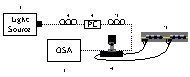
\includegraphics[width=0.8\textwidth]{fig/Setup.pdf}
    \caption{Equipment setup for measuring the six fabricated structures.}
    \label{fig:Setup}
\end{figure}

The setup consists of seven individual components as listed below: 
\begin{itemize}

    \item[1)] \textbf{Light source}\\
In our experiments we have used three different light sources; two light-emitting-diodes (LEDs), and one supercontinuum laser (see Table \ref{tablelightsources}). 

    \item[2)] \textbf{Polarisation twister}\\
Theoretically, the LEDs emit unpolarised light but with a slightly elliptical shape, and the supercontinuum laser emits unpolarised light as well. Our designs are optimised for TE-polarised light, so the light must be TE-polarised. It is not certain that all polarisations of light possess the same intensity, therefore the polarisation is aligned in order to send the highest possible intensity of light through the PC. 

    \item[3)] \textbf{Polarisation crystal (PC)}\\
This crystal only allows light with a specific angle of polarisation, cutting off all remaining light from the light source. 

    \item[4)] \textbf{Polarisation twister}\\
At this light is linearly polarised. However, the angle of polarisation must be optimal when passing through the input-waveguide of the silicon structure, which is adjusted by the second twister. This angle is found utilising a photonic crystal on the measured sample. 

    \item[5)] \textbf{Piezo motors/controllers}\\
Since the fibres must be positioned to the waveguides in the silicon structure with a precision finer than that possible with visual positioning, piezo controllers are used with the aid of the OSA to optimise the position of the fibres. 

    \item[6)] \textbf{Microscope with breadboard}\\ 
The rough positioning of the fibres is done with the aid of a microscope and some geared-down knobs, in order to get a signal through the silicon structure. The signal is optimized using the piezo controllers and the OSA. 

    \item[7)] \textbf{Optical Spectral Analyser (OSA)}\\
The OSA is used to measure the spectrum of light passed through the components. The OSA records the spectrum of light and saves the raw data on a computer. To fine-tune the position with use of piezo controllers, the light intensity (with respect to wavelength) is viewed on the OSA, and positions are optimised to maximise the intensity of light through the silicon structure accordingly. 

\end{itemize}

\subsection{Light sources used}
The first measurements were performed using a broadband light source with two simultaneous LEDs peaking at 1430 nm and 1550 nm, respectively. The LED outputs were low, so it was difficult to conclude anything from the noisy spectra recorded with the OSA, see for example Fig. \ref{fig:Lightsource1Rep}. The low-wavelength part of the spectrum (sub-1350 nm) was especially error-prone. For a reference spectrum, see Fig. \ref{fig:broadbandref} in Appendix. \\
\\
To counter the challenge with noisy spectra at low wavelengths, the next measurements were performed using a multimeter light source with 2 separate LEDs peaking at 1310 nm and 1550 nm, respectively. Only one LED could be connected to the demultiplexer at a given time, which doubled the amount of necessary measurements. It also introduced a systematic error: The fibres were manually switched between using the 1310 nm and 1550 nm LEDs, and we had to concatenate data points from separate measurements. For reference spectra, see Fig. \ref{fig:multimeterref} in Appendix.\\
\\
To obtain data without concatenation, the final measurements were performed using a supercontinuum laser as light source. The light from the supercontinuum laser is produced by nonlinear processes, and the signal prone to drifting, but the produced signal is strong, so the measurements are clear. For a reference spectrum, see Fig. \ref{fig:superKref} in Appendix. 

\begin{table}[h]
    \begin{tabular}{|clll|}
    \hline
    \textbf{\#} & \textbf{Name}                        & \textbf{Peak wavelengths [nm]} & \textbf{Characteristics}                        \\ \hline
    1               & Broadband light source      & 1430 and 1550         & 2 simultaneous light sources (2 LEDs)  \\ \hline
    2               & Multimeter light source     & 1310 or 1550          & 2 seperate light sources (2 LEDs),     \\
    ~               & ~                           & ~                     & only 1 can be connected at a time      \\ \hline
    3               & Supercontinuum light source & 1360-1500 (medium)    & produced by nonlinear processes,       \\
    ~               & ~                           & 1540-1600 (strong)    & see Fig. \ref{fig:superKref} in Appendix \\ \hline
    \end{tabular}
    \caption{Light source characteristics.}
     \label{tablelightsources}
\end{table}
